\documentclass[12pt]{article}
\usepackage[utf8]{inputenc}
\usepackage{graphicx}
\usepackage{listings}
\usepackage{wrapfig}
\usepackage{subfigure}
\usepackage{hyperref}
\usepackage{amsmath}
\usepackage[margin=1in]{geometry}

\title{\vspace{-8ex}Project Pre-Proposal:\\Browser-Based 3D Turtle}
\author{Nathan Walters\\nwalter2}
\date{\today}

\begin{document}

\maketitle

\section{Overview}

For my project, I will implement a brower-based 3D turtle graphics system using JavaScript and the HTML5 canvas. It will work very similarly to a standard 2D turtle system, with the logical extension that the turtle will be able to move along a third dimension. It will also allow the user to rotate and move the camera in 3-space so as to be able to view the turtle's drawings from different perspectives.

\section{Mathematics and Implementation}

For one of my early mini-projects, I implemented a basic 2D turtle system using JavaScript and the HTML5 canvas. It lays the groundwork for a 3D turtle; it features standard turtle move functions, a basic animation framework, the ability to add multiple turtles to a single scene, and more. Conceptually, extending the representation of the turtle into 3 dimensions isn't too difficult. A standard 2D turtle can only rotate around an axis normal to the plane in which it moves. To extend that to 3 dimensions, we can give the turtle the ability to rotate along two other axes: we can allow it to ``roll'' around its heading vector, and ``pitch'' around a third vector that is mutually perpendicular to the turtle's heading vector and normal vector.

Tavares' rotating 3D cube shows that it is possible to use pure JavaScript to project 3D scenes onto a 2D canvas. Indeed, portions of Tavare's project can be used to create a basic renderer for 3-dimensional vectors. Tavares' code will serve as the basis of my rendering engine. However, I plan to rewrite portions of his work; I have already identified some bugs with how it handles the positioning of the camera. To implement the ability to fly the camera around in the turtle's space, it will be necessary to identify and fix those issues.

\section{Applications}

In essence, a turtle graphics system is simply a means to easily generate and render vectors. Think about it: any segment drawn by a turtle is simply a magnitude (the distance the turtle moves) and a direction (the turtle's heading). Once I create a 3D turtle system, I will essentially have a means to render arbitrary 3 dimensional entities, provided they can be decomposed into line segments.

For instance, one can imagine it would be relatively easy to definte turtle movements that could trace out a wireframe cube or sphere. To draw a cube of side length $s$, we could issue the turtle the following commands: 

\begin{enumerate}
\item Move forward $s$ units, turn $90^\circ$; repeat four times (this draws a square base)
\item Pitch up $90^\circ$, move forward $s$ units, pitch down $90^\circ$ (this moves the turtle to another plane where it can draw the opposing square face)
\item Pitch down $90^\circ$, move forward $s$ units, move backwards $s$ units, pitch up $90^\circ$, move forward $s$ units, turn $90^\circ$ degrees (this draws a vertical line between the base and the opposing face, and then draws one edge of the opposign face)
\end{enumerate}

Similarly, we can easily define commands to create an approximation of a wireframe sphere. Our process for doing that will approximate the act of spinning a circle around its diameter to sweep out the surface of a sphere:

\begin{enumerate}
\item Move forward $s$ units, pitch up $10^\circ$; repeat until the turtle has turned a full $360^\circ$ (this traces out an approximation of a circle)
\item Turn $10^\circ$, repeat step 1 (this traces out another circle that is rotated slightly around the z-axis)
\item Repeat step 2 until the offset from the original circle is $180^\circ$
\end{enumerate}

It would also be possible to write a script that could make the turtle trace out the surface of a function of two variables, similar to the one illustrated below. Note that the mesh representing the surface consists of a number of connected straight lines. Given an explicit function of two variables, it should be possible to compute turtle commands that would draw out such a mesh surface.

\begin{figure}[h]
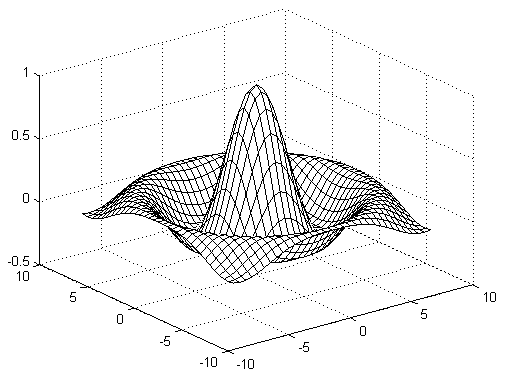
\includegraphics[scale=0.5]{3dmesh}
\centering
\end{figure}

\section{Project Steps}

\begin{enumerate}
\item Determine and understand the mathematical operations necessary to move, rotate, roll, and pitch the turtle in 3D space
\item Implement the above mathematics in JavaScript
\item Update the turtle's logic to incorporate the above mathematics to compute its movement
\item Test and debug the updated turtle logic using the existing 2D renderer (simply discard the $z$ coordinate when rendering)
\item Implement, test, and debug a new 3D renderer based on Tavares' work
\item Implement the ability to rotate and move the virtual camera within 3D space
\item Explore applications of the 3D turtle, documenting any interesting ones
\item Explore extensions to the turtle, such as the ability to render with different colors or portray depth
\end{enumerate}

\end{document}
